\documentclass[12pt]{article}
\topmargin -0.7in
\oddsidemargin -0.21in
\evensidemargin -0.21in
\textwidth=17cm
\textheight=24cm

\usepackage[utf8]{inputenc}
\usepackage[T2A]{fontenc} 
\usepackage[russian]{babel}
\usepackage{amsmath}
\usepackage{comment}

\usepackage{tikz}
\usepackage{graphicx}
\graphicspath{{./src/}}
\DeclareGraphicsExtensions{.png}

\renewcommand{\l}{\left( }
\renewcommand{\r}{\right) }
\renewcommand{\phi}{\varphi}
\newcommand{\pd}{\partial}
\newcommand{\br}[1]{\l {#1} \r}
\newcommand{\rint}{\int\limits_{-\infty}^{+\infty}}
\newcommand{\pint}{\int\limits_{-\pi}^{\pi}}
\newcommand{\jacobian}[2]{\frac{\pd \br{#1}}{\pd \br{#2}}}
\newcommand{\abs}[1]{\left| #1 \right|}

\begin{document}

\begin{center}
\large{ПРАВИТЕЛЬСТВО РОССИЙСКОЙ ФЕДЕРАЦИИ}
\vspace{2em}
\large{ФЕДЕРАЛЬНОЕ ГОСУДАРСТВЕННОЕ БЮДЖЕТНОЕ ОБРАЗОВАТЕЛЬНОЕ УЧРЕЖДЕНИЕ ВЫСШЕГО ПРОФЕССИОНАЛЬНОГО ОБРАЗОВАНИЯ \\
<<САНКТ-ПЕТЕРБУРГСКИЙ ГОСУДАРСТВЕННЫЙ УНИВЕРСИТЕТ>>\\
(СПбГУ)\\}
Кафедра физики высоких энергий и элементарных частиц\\
Направление <<Физика>>
\end{center}
\begin{figure}[h!]
\center

\includegraphics[width=.25\textwidth,clip]{eagle2.png}
\end{figure}

\begin{center}
\large{\bf ДВУХЧАСТИЧНЫЕ КОРРЕЛЯЦИИ, ВОЗНИКАЮЩИЕ ПРИ РАСПАДЕ ОДИНОЧНОЙ СТРУНЫ}
\end{center}
$$$$
$$$$
\begin{flushright}
Бакалаврская работа студента
$$$$
\_\_\_\_\_\_\_\_\_\_\_\_\_\_\_\_\_\_\_\_\_\_\_  {\bf Кравцова Павла Сергеевича} \\
\vspace{2em}
Научный руководитель: \\
\_\_\_\_\_\_\_\_\_\_\_\_\_\_\_\_\_\_\_\_\_\_  д.ф.-м.н., проф. {\bf Вечернин В. В.} \\
\vspace{2em}
Рецензент: \\
\_\_\_\_\_\_\_\_\_\_\_\_\_\_\_\_\_\_\_\_  к.ф.-м.н., ассистент {\bf Алцыбеев И. Г.} \\
\end{flushright}
$$$$

\begin{center}
\Large{
Санкт--Петербург \\
2016}
\end{center}
\thispagestyle{empty}
\newpage


\tableofcontents
\newpage

\section{Введение}
\qquad На данный момент квантовая хромодинамика - признанная теория сильных взаимодействий. Основной метод расчета в этой области, теория возмущений, не применима для расчета множественного рождения частиц в мягкой области спектра при столкновении адронов. Для подобных расчетов используются различные феноменологические модели. Одна из наиболее часто используемых моделей - модель цветных кварк-глюонных струн \cite{model1},\cite{model2},\cite{model3},\cite{model4}.

\subsection{Двухстадийное описание множественного рождения частиц}
\qquad В рамках модели цветных струн цветовое поле между кварками и бикварками заменяется струной с действием
\begin{gather}
\label{string_action}
S = \gamma \int d\sigma \int d\tau \sqrt{\br{\frac{\pd x_\mu}{\pd \tau} \frac{\pd x^\mu}{\pd \sigma}}^2 - \br{\frac{\pd x_\mu}{\pd \sigma} \frac{\pd x^\mu}{\pd \sigma}} \br{\frac{\pd x_\nu}{\pd \tau} \frac{\pd x^\nu}{\pd \tau}}}
\end{gather}
,где $\gamma=const$ - натяжение струны, $\sigma, \tau$ - переменные, параметризуюшие струну в провсранстве времени Минковского, $x^\mu=x^\mu \br{\sigma, \tau}$ - координаты струны. Это действие обеспечивает ассимптотически-линейный рост потенциальной энергии при увеличении расстояния между кварками.

До столкновения двух адронов считается, что взаимодействие есть только внутри адронов, то есть кварки одного адрона взаимодействуют только с другими кварками этого адрона. При столкновении поля-струны "перецепляются", и образуются струны между кварками и бикварками разных адронов, то есть появляются струны между обьектами летящими в противоположные стороны. Это первый этап так называемого двухстадийного механизма множественного рождения частиц. 

Далее, эти струны растягиваются и рвутся. Процесс разрыва или, как его чаще называют, фрагментации струны физически соответствует процессу рождения пары кварк-антикварк. После фрагментации образуются две новые струны, которые так же растягиваются и рвутся. Этот процесс продолжается до тех пор, пока энергии образовавшихся струн не станут порядка энергии соответствующего адрона. Тогда струны отождествляются с адронами, которые и являются конечными продуктами распада. В этом состоит второй этап двухстадийного механизма.

\subsection{"Yo-yo" струна}
\begin{figure}[h!]
\center{
\begin{tikzpicture}
% оси координат
\draw[->] (-2, 0) coordinate (O) -- +(5, 0) node [right] {$z$};
\draw[->] (O) -- +(0, 7) node [left] {$t$};
% пунктирные прямые
\draw[thick, dashed]
(0, 0) coordinate (A) -- +(-45:.5) 
(0, 0) -- +(-135:.5)
(0, 0) -- ++(45:3) -- ++(135:2) coordinate (B) -- ++(225:3) -- +(315:2) ++(45:3)
-- ++(45:3) -- ++(135:2) coordinate (C) -- ++(225:3) -- +(315:2) ++(45:3)
 -- +(45:.5) 
 +(0,0) -- +(135:.5);
% гиперболы
 \draw[thick]
(A) .. controls +(50:2.8) .. (B)
(A) .. controls +(130:1.85) .. (B)
(B) .. controls +(50:2.8) .. (C)
(B) .. controls +(130:1.85) .. (C)
(A) -- +(-55:.4)
(A) -- +(-125:.4)
(C) -- +(125:.4)
(C) -- +(55:.4);
\end{tikzpicture}
}
\caption{Движение концов струны "yo-yo" с массами (сплошная линия) и без масс (пунктирная линия).}
\label{yoyo}
\end{figure}
Действие (\ref{string_action}) задает некоторые уравнения движения для струны. Существует целый класс решений этих уравнений. Для описания столкновений адронов, как правило, используется одно из самых простых решений, так называемая струна "yo-yo". Это решение в пространстве-времени размерности 1+1 графически изображено на рис. \ref{yoyo}.

В \cite{nesterenko} показано, что движение струны, у которой массивные концы движутся со околосветовой скоростью, эквивалентно движению струны с безмассовыми концами. Для удобства будем считать концы струн безмассовыми.

\subsection{Модели фрагментации струны}
\label{fragmentation_subsection}
\begin{figure}
\center{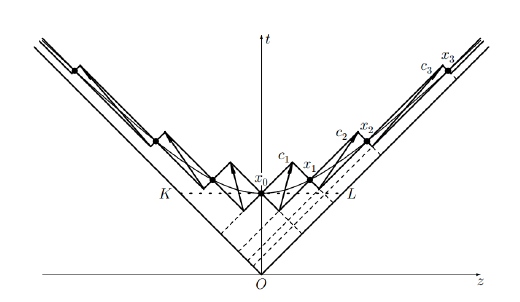
\includegraphics[width=0.8\textwidth]{fragmentation.png}}
\caption{Доминирующий процесс фрагментации струны. Иллюстрация из \cite{fragmentation_lit}}
\label{fragmentation}
\end{figure}

Cуществуют два подхода к описанию фрагментации струны. Можно описывать фрагментацию по анологии с механизмом Дж. Швингера \cite{schwinger} рождения электрон-позитронных пар в однородном электрическом поле, считая поле внутри струны приблизительно однородным. Другой подход - придумать феноменологическое правило, которое определяет вероятность разрыва в некоторой точке струны в некоторый момент времени. 

Сушествует несколько различных правил для определения вероятности фрагментации. Остановимся подробнее на правиле, истользуемом в модели Артру-Менниссиера \cite{artru}. Оно формулируется для решения "yo-yo string". Прежде всего введем координаты, которыми оно описывается. Для частиц движущихся со скоростью света удобно ввести координаты светового конуса:
\begin{gather}
b^{\pm} = \frac{1}{\sqrt 2} \br{t \pm z}
\end{gather}
Далее от них прейдем к координатам $S$ и $\Delta \eta$:
\begin{gather}
S = b^+ \cdot b^- \\
\eta = \frac{1}{2} ln \frac{b^+}{b^-}
\end{gather}
Здесь $S$ имеет смысл площади прямоугольника с длинами сторон $b^+$ и $b^-$ и сторонами парралельными осям координат светового конуса. $\eta$, так называемая быстрота, в общем случае параметризует скорость частицы или струны. Выберем начало координат так, что концы струн совпадают в точке $(t, z) = (0, 0)$. Тогда модель Артру-Меннессиера $P$ гласит, что вероятность разрыва струны зависит лишь от $S$ и не зависит от $\eta$. Она пропорциональна соответствующей площади $S$, при условии, что в данной области разрыва еще не было:
\begin{gather}
dP \br{S} = \frac{1}{S_0} \br{1 - P \br{S}} dS,
\end{gather}
где $S_0$ - параметр модели.Таким образом вероятность распада
\begin{gather}
P \br{S} = 1 - exp \br{-\frac{S}{S_0}}
\end{gather}
Из этой формулы можно вывести, что в среднем разрыв происходит с площадью $S_0$. Сделаем упрошение, и будем считать, что разрыв происходит только при $S=S_0$. Тогда все события фрагментации будут лежать на гиперболе (см. рис. \ref{fragmentation}). В \cite{fragmentation_lit} показано, что при данных предположениях струны будут рождаться равномерно распределенными по быстроте, причем разность быстрот соседних струн порядка 1 (для рождения $\pi\text{-мезона}$ $\Delta \eta = 1,5$; для $\rho-\text{мезона} - \Delta \eta = 0,75$; для нуклона $\Delta \eta = 0,63$).

И в подходе с механизмом Швингера и в модели Артру-Менниссиера получается один и тот же важный результат: в среднем частицы от фрагментации соседних частей струны попадают в соседние интервалы быстроты, а частицы от удаленных друг от друга частей струны попадают в дальние друг от друга интервалы.

\subsection{Виды корреляций}
\qquad В струнном описании процесса рассеяния существует два источника для корреляций частиц. Им соответствуют два типа корреляций: ближние и дальние. Впервые на эти типы корреляций было указанно в работах \cite{cappela}.

Ближние корреляции возникают между частицами, соответствующими струнам, которые были соседними в процессе фрагментации. Одна из струн имеет на конце некоторый кварк, образованный в результате рождения пары кварк-антикварк, в то время как другая содержит антикварк, образовавшийся в том же процессе. Из-за закона сохранения импульса кварк и антикварк имеют скоррелированые импульсы, поэтому импульсы частиц тоже оказываются скоррелированными. Так-как подобные корреляции имеют место между соседними струнами, соосветствуюшие частицы имеют близкие по величине быстроты, другими словами явление наблюдается в близких быстротных окнах.

Дальние корреляции, наоборот, наблюдаются в разнесенных по быстроте окнах. Они обусловленны в первую очередь флуктуациями числа образовавшихся струн. В работах \cite{fusion1}, \cite{fusion2} была предложена модификация струнной модели, учитывающая процессы слияния струн, перед началом второго этапа двухстадийного механизма.
Слияние струн так же приводит к дальним корреляциям, что подробно изучалось в работах \cite{fusion_corr1}, \cite{fusion_corr2}, \cite{fusion_corr3}, \cite{fusion_corr4}.

В данной работе исследуются именно ближние корреляции, возникающие в одиночной струне.


\section{Цель работы}
\begin{figure}
\center{
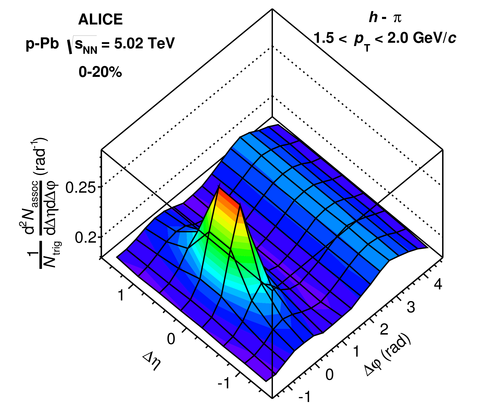
\includegraphics[width=0.7\textwidth]{main.png}
}
\caption{Распределение по разности быстрот $\Delta \eta$ и углу разлета $\Delta \phi$ частиц в процессе множественного рождения ($1.5 Gev < p_T < 2.0 GeV$). График из \cite{exp_data}}
\label{main}
\end{figure}

\qquad На рис. \ref{main} изображена характерная двухчастичная функция распределения зависящая от разности быстрот $\Delta \eta$ и углу разлета $\Delta \phi$ частиц, образовавшихся после столкновения. На нем выделяются два пика. Острый пик с центром в точке $(\Delta \eta, \Delta \phi) \approx (0, 0)$ говорит о том, что образуется много пар частиц летящих в одну сторону с одной быстротой. Это объясняется тем, что в после фрагментации образуетются не только частицы с основным состоянием, но и частицы с резонансным состоянием. Подобные резонансы до улавливания детекторами сами распадаются на две и более стабильные частицы. Детекторы регистрируют именно эти стабильные частицы, которые разумеется будут иметь схожие быстроты и направления. Для процессов образования и последующего распада резонансов в рамках струнного подхода существуют различные модели. Например, в генераторе событий VENUS используется так называемая модель AMOR (Artru-Mennessier off-shell resonance model) \cite{venus}. Это расширение модели Артру-Меннессиера в которой модифицируется формула для вероятности распада струны так, чтобы учесть возможное рождение резонансов. В данной работе подобные процессы не расматриваются. 

Второй пик, или скорее хребет, сильно "размазан" по быстроте и имеет центр на линии $\Delta \phi \approx 3$. Это так называемый задний ридж (back ridge). 
\textbf{Целью нашей работы} является обьяснить его образование в рамках струнного подхода. Мы покажем, что наличие этого пика означает наличие ближних корреляций в процессе фрагментации одиночной струны, которые обусловлены локальным законом сохранения импульса.

\section{Модель одиночной струны}
\begin{figure}
\center{
\begin{tikzpicture}
% оси X, Y, Z
\fill (1, 1) coordinate (O);
\draw[thick, ->] (O) node [below] {$O$} -- +(90:1) node [right] {$x$};
\draw[thick, ->] (O) node [below] {$O$} -- +(225:.5) node [left] {$y$};
\draw[thick, ->] (O) node [below] {$O$} -- +(0:1) node [right] {$z$};

%труба
\draw[very thick, gray] (0, .5) -- ++(1.5, 0) ++(1.5, 0) -- ++(9, 0) ++(1.5, 0) -- ++(1.5, 0);
\draw[very thick, gray, dashed] (1.5, .5) -- ++(1.5, 0) ++(9, 0) -- ++(1.5, 0);
\draw[very thick, gray] (0, -.5) -- ++(1.5, 0) ++(1.5, 0) -- ++(9, 0) ++(1.5, 0) -- ++(1.5, 0);
\draw[very thick, gray, dashed] (1.5, -.5) -- ++(1.5, 0) ++(9, 0) -- ++(1.5, 0);
\draw[very thick, gray] (0, .5) arc (90:270:0.25 and 0.5);
\draw[very thick, gray, densely dashed] (0, -.5) arc (270:450:0.25 and 0.5);
\draw[very thick, gray] (15, 0) ellipse (0.25 and 0.5);

% палочки между кварками
\draw[ultra thick]
(0.7, 0) coordinate (QM) -- +(-5:0.85)
(4.5, -.2) coordinate (AQ1) -- +(177:1.6)
(4.5, .2) coordinate (Q1) -- (7.5, .3) coordinate (AQ2)
(7.5, -.3) coordinate (Q2) -- (10.5, .2) coordinate (AQ3)
(10.5, -.2) coordinate (Q3) -- +(4:1.5)
(14.55, 0) coordinate(AQN) -- +(176:1.1) ;

% стрелочки
\def\impangle{40}
\draw[thick, ->] (Q1) -- +(\impangle :1.5) node [right] {$\vec{q_1}$};
\draw[thick, ->] (AQ1) -- +(\impangle + 180:1.5) node [left] {$\vec{\bar{q_1}}$};
\draw ++(Q1) -- +(90:1) +(\impangle:.5) arc (\impangle:90:.5) node [above right] {$\phi_1$};
\def\impangle{-70}
\draw[thick, ->] (Q2) -- +(\impangle :1.0) node [right] {$\vec{q_2}$};
\draw[thick, ->] (AQ2) -- +(\impangle + 180:1.0) node [left] {$\vec{\bar{q_2}}$};
\draw ++(Q2) -- +(90:1) +(\impangle:.5) arc (\impangle:90:.5) node [right] {$\ \phi_2$};
\def\impangle{-30}
\draw[thick, ->] (Q3) -- +(\impangle :2.0) node [right] {$\vec{q_3}$};
\draw[thick, ->] (AQ3) -- +(\impangle + 180:2.0) node [left] {$\vec{\bar{q_3}}$};
\draw ++(Q3) -- +(90:1) +(\impangle:.5) arc (\impangle:90:.5) node [right] {$\ \phi_3$};

% кварки
\draw[fill=gray] (QM) circle (0.15) node [left] {$\vec{q}_{-m}$};
\draw[fill=white] (AQ1) circle (0.15);
\draw[fill=gray] (Q1) circle (0.15);
\draw[fill=white] (AQ2) circle (0.15);
\draw[fill=gray] (Q2) circle (0.15);
\draw[fill=white] (AQ3) circle (0.15);
\draw[fill=gray] (Q3) circle (0.15);
\draw[fill=white] (AQN) circle (0.15) node [right] {$\ \vec{\bar{q_n}}$};
\end{tikzpicture}
}
\caption{Модель цветной кварк-глюонной струны}
\label{string}
\end{figure}

В соответствии с секцией \ref{fragmentation_subsection} мы считаем, что образовавшиеся струны имеют одинаковую длину. Кроме того считаем, что разность быстрот для соседних струн одинакова и $\Delta \eta \approx 1$. Для краткости будем называть и кварки, и бикварки просто кварками. Антикварком для бикварка будем считать кварк, способный дополнить его до адрона. Обозначим поперечные импульсы кварков (антикварков) $\vec{q_i}, i = -m, -m + 1, ... , n$ и $\vec{\bar{q_i}}$ - поперечные импульсы парных к ним антикварков (кварков) (см. рис. \ref{string}). Фиксируем ось $Ox$ перпендикулярную струне и будем отсчитывать направления поперечных импульсов $\phi_i$ от неё. Поперечные импульсы образовавшихся адронов обозначим $\vec{p_i}$. Тогда в наших обозначениях $\Delta \phi$ - угол между векторами $\vec{p_i}$ и $\vec{p_j}$.

Закон сохранения импульса накладывает ограничения на процессы рождения пар кварк-антикварк. Мы считаем, что суммарный импульс пары должен быть равен нулю, следовательно
\begin{gather}
\vec{\bar{q_i}} = -\vec{q_i} \\
\vec{p_i} = \vec{q}_{i+1} + \vec{\bar{q_i}} = \vec{q}_{i+1} - \vec{q_i}
\end{gather}
Таким образом, величины $q_i$ и $\phi_i$ однозначно задают все поперечные координаты модели.

Будем обозначать функцию распределения величины $a$ в точке $a_0$ как $\rho_a \br{a_0}$. Нас будут интересовать функции распределения $\rho_{\Delta \phi} \br{\Delta \phi'}$ и $\rho_{p_i} \br{p_i'}$. Мы будем искать их на основе различных предположений о распределении величин $q_i$ и $\phi_i$.

\section{Вычисление функций распределения}
В работе предполагается известными распределения по направлениям разлета кварков $\rho_{\phi_i}$ и по величине поперечного импульса $\rho_{q_i}$. Из них находятся распределение по углу разлета $\rho_{\Delta \phi}$ соседних адронов (адроны с номерами 1 и 2) и распределение по величине импульса $\rho_p$ одного адрона (для определенности рассматриваем адрона с номером 1 т. е. $p = p_1$). Рассматриваются два варианта распределений импульсов кварков:
\begin{itemize}
\item "Константный" случай, когда $q_i$ фиксированно и одинаково для всех кварков: $q_i = q_0, \rho_{q_i} \br{q} = \delta \br{q - q_0}$.
\item "Гауссовый" случай, когда $\rho_{q_i} \br{q} = \frac{q}{2 q_0^2} exp \br{-\frac{q^2}{q_0^2} }$.
\end{itemize}
В обоих случаях направления разлета считаются распределенными равномерно: \newline $\rho_{\phi_i} \br{\phi_i} = \frac{1}{2\pi}$ ($\phi_i \in \left[ -\pi, \pi \right]$). В вычислениях используем обозначение для якобиана перехода от координат $x_1,\ldots , x_n$ к координатам $y_1,\ldots ,\ y_n$ - $\jacobian{y_1,\ldots , y_n}{x_1,\ldots , x_n}$. Иногда нам будет удобнее использовать декартовы координаты:
\begin{gather}
q_i^x = q_i \cdot cos \l \phi_i \r,\quad q_i^y = q_i \cdot sin \br{ \phi_i}
\end{gather}

\subsection{Распределение по импульсу в константном случае}
Элементарные события нумеруются парами $\l \phi_1, \phi_2 \r$. Поперечный импульс мезона
\begin{eqnarray}
p \br{\phi_1, \phi_2} = \sqrt{\br{\vec{q_2} - \vec{q_1}}^2} = \sqrt{q_2^2 + q_1^2 - 2 q_1 q_2 cos \br{\phi_2 - \phi_1}} = \nonumber \\
= q_0 \sqrt{2 \br{1 - cos \br{ \phi_2 - \phi_1 }}} = 2 q_0 \left|{sin \br{\frac{\phi_2 - \phi_1}{2}}}\right|
\end{eqnarray}
По определению функция распределения величины $p$ - это вероятность того, что величина $p$ имеет значение $p'$:
\begin{eqnarray}
\rho_p \br{p'} = \pint \rho_{\phi_1} \br{\phi_1} d\phi_1 \pint \rho_{\phi_2} \br{\phi_2} d\phi_2 \cdot \delta \br{p' - p(\phi_1, \phi_2)} \nonumber \\
= \frac{1}{\br{2\pi}^2} \pint \pint d\phi_1 d\phi_2 \cdot \delta \br{p' - p(\phi_1, \phi_2)}
\end{eqnarray}
Сделаем замену
\begin{eqnarray}
\begin{cases}
\theta_1 = \frac{\phi_1 + \phi_2}{2} \\
\theta_2 = \frac{\phi_2 - \phi_1}{2}
\end{cases}
\nonumber
\end{eqnarray}
Якобиан преобразования
\begin{eqnarray}
\jacobian{\phi_1, \phi_2}{\theta_1, \theta_2} = \br{\jacobian{\theta_1, \theta_2}{\phi_1, \phi_2}}^{-1} = \br{det 
\begin{pmatrix}
\quad\frac{1}{2} & \frac{1}{2} \\
-\frac{1}{2} & \frac{1}{2}
\end{pmatrix}
}^{-1} = 2
\end{eqnarray}
Заметим, что $p$ зависит только от $\theta_2$ и по переменной $\theta_1$ можно проинтегрировать
\begin{eqnarray}
\rho_p \br{p'} = \frac{1}{\br{2\pi}^2} \pint d\theta_2 \int\limits_{-\pi + \abs{\theta_2}}^{\pi - \abs{\theta_2}} d\theta_1 \ \abs{\jacobian{\phi_1, \phi_2}{\theta_1, \theta_2}}\cdot \delta \br{p' - p \br{\theta_2}} = \nonumber \\
= \frac{1}{\pi^2} \pint d\theta_2 \ \br{\pi - \abs{\theta_2}} \cdot \delta \br{p' - p \br{\theta_2}}
\end{eqnarray}
Кроме того $p\br{-\theta_2} = p\br{\pi - \theta_2} = p\br{\theta_2}$, поэтому
\begin{gather}
\rho_p \br{p'} = \frac{2}{\pi^2} \int\limits_0^\pi d\theta_2 \ \br{\pi - \theta_2} \cdot \delta \br{p' - p \br{\theta_2}} = \nonumber \\
= \frac{2}{\pi^2} \int\limits_0^{\pi/2} d\theta_2 \br{\pi - \theta_2} \cdot \delta \br{p' - p \br{\theta_2}} + 
\underbrace{\frac{2}{\pi^2}\int\limits_{\pi/2}^\pi d\theta_2 \br{\pi - \theta_2} \cdot \delta \br{p' - p \br{\theta_2}} }_{
\begin{matrix}
\theta_2'=\pi - \theta_2 \\
\frac{2}{\pi^2}\int\limits_0^{\pi/2} d\theta_2' \theta_2' \cdot \delta \br{p' - p \br{\theta_2'}}
\end{matrix}
} = \\
\frac{2}{\pi} \int\limits_0^{\pi/2} d\theta_2 \cdot \delta \br{p' - p \br{\theta_2}}
\nonumber
\end{gather}
Наконец, перейдем к переменной $p = 2 q_0 \ sin \theta_2$
\begin{eqnarray}
\rho_p \br{p'} = \frac{2}{\pi} \int\limits_0^{2 q_0} dp \frac{1}{\pd p/\pd \theta_2} \cdot \delta \br{p' - p} = \frac{2}{\pi} \int\limits_0^{2 q_0} \frac{dp \cdot \delta \br{p' - p}}{\sqrt{\br{2 q_0}^2 -p^2}} = \frac{2}{\pi\sqrt{\br{2 q_0}^2 -p'^2}}
\end{eqnarray}

\subsection{Распределение по $\Delta \phi$ в константном случае}
$\Delta \phi$ - угол между векторами $\vec{p_1}$ и $\vec{p_2}$, поэтому
\begin{eqnarray}
cos \Delta \phi = \frac{\vec{p_1} \cdot \vec{p_2}}{p_1 p_2}
\end{eqnarray}
В нашем случае
\begin{eqnarray}
\vec{p_1} = q_0 \
\begin{pmatrix}
cos \phi_2 - cos \phi_1 \\
sin \phi_2 - sin \phi_1
\end{pmatrix}
,\quad\vec{p_2} = q_0 \
\begin{pmatrix}
cos \phi_3 - cos \phi_2 \\
sin \phi_3 - sin \phi_2
\end{pmatrix}
\end{eqnarray}
Следовательно
\begin{gather}
cos \Delta \phi = \nonumber \\
 =\frac{\br{cos \phi_2 - cos \phi_1}\br{cos \phi_3 - cos \phi_2} + \br{sin \phi_2 - sin \phi_1} \br{sin \phi_3 - sin \phi_2} }{\br{\br{ \br{cos \phi_2 - cos \phi_1}^2 + \br{sin \phi_2 - sin \phi_1}^2} \br{ \br{cos \phi_3 - cos \phi_2}^2 + \br{sin \phi_3 - sin \phi_2}^2}}^{1/2}} = \nonumber \\
= \frac{1}{2} \frac{cos\br{\phi_2 - \phi_1} + cos\br{\phi_3 - \phi_2} - cos\br{\phi_3 -\phi_1} - 1}{\br{\br{1 - cos \br{\phi_2-\phi_1}} \br{1 - cos\br{\phi_3 - \phi_2}}}^{1/2}} = \nonumber \\
= \frac{1}{2} \frac{sin^2\frac{\phi_3 -\phi_1}{2} - sin^2 \frac{\phi_3 -\phi_2}{2} - sin^2 \frac{\phi_2 -\phi_1}{2}}{\abs{sin\frac{\phi_2 -\phi_1}{2} sin\frac{\phi_3 - \phi_2}{2}}} = \nonumber\\
=sign\br{sin\frac{\phi_3 -\phi_2}{2} sin\frac{\phi_2-\phi_1}{2}} cos\frac{\phi_3 - \phi_1}{2}
\end{gather}
где $sign\br{x} = \begin{cases} 1,\quad \text{если} x \ge 0 \\ -1,\quad \text{если} x < 0\end{cases}$. \newline
Ясно что из этого выражения можно найти лишь $\abs{\Delta \phi}$. С учетом того, что $\phi_i \in \left[-\pi, \pi \right]$, получаем
\begin{eqnarray}
\label{DeltaPhi}
\abs{\Delta \phi} = 
\begin{cases}
\abs{\frac{\phi_3 - \phi_1}{2}},\quad \text{если} \br{\phi_3 -\phi_2} \br{\phi_2 -\phi_1} \ge 0 \\
\pi - \abs{\frac{\phi_3 - \phi_1}{2}},\quad \text{если} \br{\phi_3 -\phi_2} \br{\phi_2 -\phi_1} < 0
\end{cases}
\end{eqnarray}
 Найдем функцию распределения величины $\abs{\Delta \phi}$. Элементарные события нумеруются наборами $\br{\phi_1, \phi_2, \phi_3}$. Выражение (\ref{DeltaPhi}) не изменяется при перестановки $\phi_1$ и $\phi_3$ местами, поэтому
\begin{gather}
\rho_{\abs{\Delta \phi}} \br{\alpha} = \pint \rho_{\phi_1} d\phi_1 \pint \rho_{\phi_2} d\phi_2 \pint \rho_{\phi_3} d\phi_3 \cdot \delta \br{\alpha - \abs{\Delta \phi} \br{\phi_1, \phi_2, \phi_3}} = \nonumber \\
\frac{2}{\br{2\pi}^3} \pint \pint d\phi_2 d\phi_3 \int\limits_{-\pi}^{\phi_3} d\phi_1 \cdot \delta \br{\alpha - \abs{\Delta \phi} \br{\phi_1, \phi_2, \phi_3}} = \\
=\frac{1}{4\pi^3} \pint d\phi_3 \int\limits_{-\pi}^{\phi_3} d\phi_1 \left[ \int\limits_{\phi_1}^{\phi_3} d\phi_2 \cdot \delta \br{\alpha - \frac{\phi_3 - \phi_1}{2}} + \int\limits_{\phi_2 \in \left[ -\pi, \phi_1 \right] \cup \left[ \phi_3, \pi\right]} d\phi_2 \cdot \delta \br{\alpha - \pi + \frac{\phi_3 -\phi_1}{2}} \right] = \nonumber \\
=\frac{1}{4\pi^3} \pint d\phi_3 \int\limits_{-\pi}^{\phi_3} d\phi_1 \left[ \br{\phi_3 -\phi_1} \cdot \delta \br{\alpha - \frac{\phi_3 - \phi_1}{2}} + \br{2\pi - \br{\phi_3 - \phi_1}} d\phi_2 \cdot \delta \br{\alpha - \pi + \frac{\phi_3 -\phi_1}{2}} \right] \nonumber
\end{gather}
Сделаем замену переменных
\begin{eqnarray}
\begin{cases}
\theta = \frac{\phi_3 -\phi_1}{2} \\
\phi_1 = \phi_1
\end{cases}
\end{eqnarray}
Якобиан преобразования
\begin{eqnarray}
\jacobian{\phi_1, \phi_3}{\phi_1, \theta} = \frac{1}{\jacobian{\phi_1, \theta}{\phi_1, \phi_3}} = \frac{1}{\pd \theta / \pd \phi_3} = 2
\end{eqnarray}
\begin{eqnarray}
\rho_{\abs{\Delta \phi}} \br{\alpha} = \frac{1}{4\pi^3} \int\limits_0^\pi d\theta \int\limits_{-\pi}^{\pi - 2\theta} d\phi_1 \jacobian{\phi_1, \phi_3}{\phi_1, \theta} \br{2\theta \delta \br{\theta - \alpha} + \br{2\pi - 2\theta} \cdot \delta \br{\theta - \br{\pi - \alpha}}} = \nonumber \\
= \frac{2}{\pi^3} \int\limits_0^\pi d\theta \br{\pi - \theta} \br{\theta \delta \br{\theta - \alpha} + \br{\pi - \theta} \cdot \delta \br{\theta - \br{\pi - \alpha}}} = \frac{2\alpha}{\pi^2}
\end{eqnarray}
Так как распределение $\Delta \phi$ симметрично, получаем
\begin{eqnarray}
\rho_{\Delta \phi} \br{\Delta \phi} = \frac{\abs{\Delta \phi}}{\pi^2}
\end{eqnarray}

\subsection{Распределение по импульсу в гауссовом случае}
Ищем распределение величины
\begin{eqnarray}
p = \sqrt{\br{q_2^x - q_1^x}^2 + \br{q_2^y - q_1^y}^2}
\end{eqnarray}
Элементарные события задаются наборами $\br{q_1^x, q_1^y, q_2^x, q_2^y}$.
\begin{eqnarray}
\rho_p \br{p'} = \br{q_0 \sqrt\pi}^{-4} \rint\rint\rint\rint dq_1^x dq_1^y dq_2^x dq_2^y  \ exp \br{-\frac{1}{q_0^2} \br{\br{q_1^x}^2 + \br{q_1^y}^2 + \br{q_2^x}^2 + \br{q_2^y}^2}} \cdot \nonumber \\
\cdot \delta \br{p' - p\br{q_1^x, q_1^y, q_2^x, q_2^y}}
\end{eqnarray}
Сделаем замену
\begin{eqnarray}
\begin{cases}
p^x = q_2^x - q_1^x \\
p^y = q_2^y - q_1^y \\
q_2^x = q_2^x \\
q_2^y = q_2^y
\end{cases}
\end{eqnarray}
Якобиан преобразования
\begin{eqnarray}
\jacobian{q_1^x, q_1^y, q_2^x, q_2^y}{p^x, p^y, q_2^x, q_2^y} = \br{\jacobian{p^x, p^y, q_2^x, q_2^y}{q_1^x, q_1^y, q_2^x, q_2^y}}^{-1} = \br{\jacobian{p^x, p_y}{q_1^x, q_1^y}}^{-1} = \br{ det
\begin{pmatrix}
-1 & 0 \\
0 & -1
\end{pmatrix}
}^{-1} = 1
\end{eqnarray}
\begin{eqnarray}
\rho_p \br{p'} = \br{q_0 \sqrt\pi}^{-4} \rint \rint dp^x dp^y \cdot \delta \br{p' - \sqrt{\br{p^x}^2 + \br{p^y}^2}} \cdot \nonumber \\
\cdot \rint \rint dq_2^x dq_2^y \ exp \br{-\frac{1}{q_0^2} \left[ 2 \br{q_2^x - \frac{p^x}{2}}^2 + \frac{\br{p^x}^2}{2} + 2 \br{q_2^y - \frac{p^y}{2}}^2 + \frac{\br{p^y}^2}{2} \right]} = \nonumber \\
= \br{q_0 \sqrt{2\pi}}^{-2} \rint \rint dp^x dp^y \cdot \delta \br{p' - \sqrt{\br{p^x}^2 + \br{p^y}^2}} \ exp \br{-\frac{\br{p^x}^2 + \br{p^y}^2}{2q_0^2}} \nonumber \\
= 2 \cdot \br{q_0 \sqrt{\pi}}^{-2} \int\limits_0^\infty \int\limits_0^\infty dp^x dp^y \cdot \delta \br{p' - \sqrt{\br{p^x}^2 + \br{p^y}^2}} \ exp \br{-\frac{\br{p^x}^2 + \br{p^y}^2}{2q_0^2}}\end{eqnarray}
Сделаем замену декартовых координат $\br{p^x, p^y}$ на полярные $\br{p, \alpha}$ и проинтегрируем по углу $\alpha$.
\begin{eqnarray}
\rho_p \br{p'} = \frac{1}{q_0^2} \int\limits_0^\infty dp p \cdot \delta \br{p' - p} \ exp \br{-\frac{p^2}{2q_0^2}} = \frac{p' \ e^{-\frac{p'^2}{2q_0^2}}}{q_0^2}
\end{eqnarray}

\subsection{Распределение по $\Delta \phi$ в гауссовом случае}
Ищем распределение $\Delta \phi$ на основе формулы
\begin{eqnarray}
cos \Delta \phi = \frac{\vec{p_1} \cdot \vec{p_2}}{p_1 p_2}
\end{eqnarray}
Элементарные события нумеруются наборами $\br{q_1^x, q_1^y, q_2^x, q_2^y, q_3^x, q_3^y}$. Вначале найдем распределение величины
\begin{eqnarray}
\gamma = cos \Delta \phi,\quad \gamma \in \left[ -1, 1 \right]
\end{eqnarray}
Распределение этой величины
\begin{gather}
\rho_\gamma \br{\gamma'} = \rint \rho_{q_1^x} \br{q_1^x} dq_1^x \rint \rho_{q_1^y} \br{q_1^y} dq_1^y \rint \rho_{q_2^x} \br{q_2^x} dq_2^x \rint \rho_{q_2^y} \br{q_2^y} dq_2^y \rint \rho_{q_3^x} \br{q_3^x} dq_3^x \cdot \nonumber \\
\label{BigIntegral}
\rint \rho_{q_3^y} \br{q_3^y} dq_3^y \cdot \delta \br{\gamma' - \gamma \br{q_1^x, q_1^y, q_2^x, q_2^y, q_3^x, q_3^y}} = \\
= \br{q_0 \sqrt\pi}^{-6} \rint \rint \rint dq_1^y dq_2^y dq_3^y \ exp \br{-\frac{1}{q_0^2} \br{\br{q_1^y}^2 +\br{q_2^y}^2 + \br{q_3^y}^2}} \cdot \nonumber \\
\cdot \underbrace{\left[ \rint \rint \rint dq_1^x dq_2^x dq_3^x \ exp \br{-\frac{1}{q_0^2} \br{\br{q_1^x}^2 +\br{q_2^x}^2 + \br{q_3^x}^2}} \cdot \delta \br{\gamma' - \gamma \br{q_1^x, q_1^y, q_2^x, q_2^y, q_3^x, q_3^y}} \right]}_{I_x}\nonumber
\end{gather}
В интеграле $I_x$ сделаем замену
\begin{eqnarray}
\begin{cases}
p_1^x = q_2^x - q_1^x \\
q_2^x = q_2^x \\
p_2^x = q_3^x - q_2^x \\
\end{cases} \quad
\jacobian{q_1^x, q_2^x, q_3^x}{p_1^x, q_2^x, p_2^x} = \br{\jacobian{p_1^x, p_2^x}{q_1^x, q_3^x}}^{-1} = -1
\end{eqnarray}
и проинтегрируем по $q_2^x$
\begin{gather}
I_x = \rint \rint dp_1^x dp_2^x \ exp \br{-\frac{2}{3q_0^2} \br{\br{p_1^x}^2 + \br{p_2^x}^2 + p_1^x p_2^x}} \cdot \nonumber \\
\cdot \rint dq_2^x \ exp \br{-\frac{3\br{q_2^x + \br{p_2^x - p_1^x}/3}^2}{q_0^2}} \cdot \delta \br{\gamma' - \gamma \br{p_1^x, p_2^x, q_1^y, q_2^y, q_3^y}} = \\
= q_0\sqrt{\frac{\pi}{3}} \rint \rint dp_1^x dp_2^x \ exp \br{-\frac{2}{3q_0^2} \br{\br{p_1^x}^2 + \br{p_2^x}^2 + p_1^x p_2^x}} \cdot \delta \br{\gamma' - \gamma \br{p_1^x, p_2^x, q_1^y, q_2^y, q_3^y}} \nonumber
\end{gather}
Теперь в формуле (\ref{BigIntegral}) проделаем аналогичную замену для $y$-координат. В итоге получим
\begin{gather}
\rho_\gamma \br{\gamma'} = \frac{1}{3 \pi^2 q_0^4} \rint \rint \rint \rint dp_1^x dp_2^x dp_1^y dp_2^y \cdot \nonumber \\
\cdot exp \br{-\frac{2}{3q_0^2} \br{\br{p_1^x}^2 + \br{p_2^x}^2 + \br{p_1^y}^2 + \br{p_2^y}^2 + p_1^x p_2^x + p_1^y p_2^y}} \cdot \delta \br{\gamma' - \gamma \br{p_1^x, p_2^x, p_1^y, p_2^y}}
\end{gather}
Сделаем замену
\begin{gather}
\begin{cases}
\label{Zamena}
p_1 = \sqrt{\br{p_1^x}^2 + \br{p_1^y}^2} \\
p_2 = \sqrt{\br{p_2^x}^2 + \br{p_2^y}^2} \\
m = p_1^x p_2^x + p_1^y p_2^y \\
p_2^y = p_2^y \\
\end{cases} \\
\abs{\jacobian{p_1^x, p_1^y, p_2^x, p_2^y}{m, p_1, p_2, p_2^y}} = \abs{\jacobian{m, p_1, p_2}{p_1^x, p_1^y, p_2^x}}^{-1} = \abs{ det
\begin{pmatrix}
p_2^x & \frac{p_1^x}{p_1} & 0 \\
p_2^y & \frac{p_1^y}{p_1} & 0 \\
p_1^x & 0 & \frac{p_2^x}{p_2} \\
\end{pmatrix}
}^{-1} = \nonumber \\
 = \abs{\frac{p_2^x\br{p_2^x p_1^y - p_2^y p_1^x}}{p_1 p_2}}^{-1} = \frac{1}{\sqrt{\br{p_2^2 - \br{p_2^y}^2} \br{1 - \br{\frac{m}{p_1 p_2}}^2}}}
\end{gather}
Это замена не взаимно-одназначная, но ее можно сделать такой. Разобьем исходный интеграл на четыре интеграла с областями интегрирования, различающимеся знаками величин $p_x^2$ и $\br{p_2^x p_1^y - p_2^y p_1^x}$. В каждом из них замена (\ref{Zamena}) будет взаимно-однозначной, и результат будет одинаков для обоих интегралов, поэтому все сведется к появлению множителя 4
\begin{gather}
\rho_\gamma \br{\gamma'} = \frac{4}{3 \pi^2 q_0^4} \int\limits_0^{+\infty} \int\limits_0^{+\infty} dp_1 dp_2 \int\limits_{-p_1 p_2}^{p_1 p_2} dm \frac{exp \br{-\frac{2}{3q_0^2}\br{p_1^2 + p_2^2 + m}}}{\sqrt{1 - \br{\frac{m}{p_1 p_2}}^2}} \underbrace{\int\limits_{-p_2}^{p_2} \frac{dp_2^x}{\sqrt{p_2^2 - \br{p_2^y}^2}}}_\pi \cdot \delta \br{\gamma' - \frac{m}{p_1 p_2}}
\end{gather}
Перейдем от переменной $m$ к переменной $\gamma = \frac{m}{p_1 p_2}$
\begin{gather}
\rho_\gamma \br{\gamma'} = \frac{4}{3 \pi q_0^4} \int\limits_0^{+\infty} \int\limits_0^{+\infty} dp_1 dp_2 \int\limits_{-1}^{1} d\gamma \frac{p_1 p_2 \ exp \br{-\frac{2}{3q_0^2}\br{p_1^2 + p_2^2 + p_1 p_2 \gamma}}}{\sqrt{1 - \gamma^2}} \cdot \delta \br{\gamma' - \gamma}
\end{gather}
Теперь заменим переменные $p_1, p_2$ на $p \in \left[ 0, +\infty \r, \theta \in \left[ 0, \pi \right]$
\begin{gather}
\begin{cases}
p \ cos \frac{\theta}{2} = p_1 \\
p \ sin \frac{\theta}{2} = p_2 \\
\end{cases} \quad
\jacobian{p_1, p_2}{p, \theta} = det
\begin{pmatrix}
cos \frac{\theta}{2} & sin \frac{\theta}{2} \\
- \frac{p}{2} \ sin \frac{\theta}{2} & \frac{p}{2} \ cos \frac{\theta}{2} \\
\end{pmatrix}
= \frac{p}{2}
\end{gather}
Теперь можно проинтегрировать по $p$
\begin{gather}
\rho_\gamma \br{\gamma'} = \frac{1}{3\pi q_0^4} \int\limits_0^\pi sin \theta \ d\theta \int\limits_{-1}^1 d\gamma \ \frac{\delta \br{\gamma' - \gamma}}{\sqrt{1 - \gamma^2}} \int\limits_0^{+\infty} p^3 \ dp \ exp \br{-\frac{2}{3q_0^2} p^2 \br{1 + \frac{\gamma}{2} \ sin \theta}} = \nonumber \\
= \frac{3}{8 \pi} \int\limits_0^\pi d\theta \int\limits_{-1}^1 d\gamma \ \frac{\delta \br{\gamma' - \gamma}}{\sqrt{1 - \gamma^2}} \cdot \frac{sin \theta}{\br{1 + \frac{\gamma}{2} \ sin \theta}^2} = \nonumber \\
= -\frac{3}{8 \pi} \int\limits_{-1}^1 d\gamma \ \frac{\delta \br{\gamma' - \gamma}}{\sqrt{1 - \gamma^2}} \cdot \frac{d}{d \br{\gamma / 2}} \br{\int\limits_0^\pi \frac{d\theta}{1 + \frac{\gamma}{2} \ sin \theta}} = \nonumber \\
= \frac{3}{4 \pi} \int\limits_{-1}^1 d\gamma \ \frac{\delta \br{\gamma' - \gamma}}{\sqrt{1 - \gamma^2}} \cdot   \frac{\sqrt{1 - \br{\gamma / 2}^2} - \br{\gamma / 2} \ arccos \br{\gamma / 2}}{\br{1 - \br{\gamma/2}^2}^{3/2}} = \nonumber \\
= \frac{3}{4 \pi} \cdot \frac{1}{\sqrt{1 - \gamma'^2}} \cdot   \frac{\sqrt{1 - \br{\gamma' / 2}^2} - \br{\gamma' / 2} \ arccos \br{\gamma' / 2}}{\br{1 - \br{\gamma'/2}^2}^{3/2}}
\end{gather}
Здесь использованы формулы для интегралов
\begin{gather}
\int\limits_0^{+\infty} dx \ x^3 e^{-\alpha x^2} = \frac{1}{2\alpha^2} \\
\int\limits_0^\pi \frac{d\theta}{1 + a \ sin \theta} = \frac{2}{\sqrt{1 - a^2}} \cdot arctg \frac{a + tg \br{\theta / 2}}{\sqrt{1 - a^2}} \Big{|}_0^\pi = \frac{2 \ arccos \br{a}}{\sqrt{1 - a^2}},\quad \text{при} \abs{a} < 1
\end{gather}
Теперь найдем распределение по углу $\Delta \phi$
\begin{gather}
\abs{\Delta \phi} = arccos \gamma
\end{gather}
Ясно, что распределение по $\abs{\Delta \phi}$ отличается от распределения по $\gamma$ на множитель $\abs{\frac{\pd \gamma}{\pd \theta}} = \abs{sin \theta} = \sqrt{1 - \gamma^2}$. Кроме того распределение по $\Delta \phi$ должно быть симметрично, поэтому в итоге получаем
\begin{gather}
\rho_{\Delta \phi} \br{\Delta \phi} = \frac{3}{8 \pi} \cdot \frac{\sqrt{1 - \br{\gamma / 2}^2} - \br{\gamma / 2} \ arccos \br{\gamma / 2}}{\br{1 - \br{\gamma/2}^2}^{3/2}}, \quad \text{где} \ \gamma = cos \Delta \phi
\end{gather}

\subsection{Компьютерное вычисление функций распределения}
Для подтверждения формул для вычисления функций распределения была написана программа, использующая метод Монте-Карло. В ней генерировалось $N = 10^4,10^5$ событий и строились гистограммы исследуемых величин (рис. \ref{const_fig}, \ref{gauss_fig}).

\section{Результаты}
\subsection{Константный случай}
В случае фиксированой величины импульса кварков импульс мезона и угол разлета определяются выражениями
\begin{eqnarray}
p =  2 q_0 \left|{sin \br{\frac{\phi_2 - \phi_1}{2}}}\right| \\
\abs{\Delta \phi} = 
\begin{cases}
\abs{\frac{\phi_3 - \phi_1}{2}},\quad \text{если} \br{\phi_3 -\phi_2} \br{\phi_2 -\phi_1} \ge 0 \\
\pi - \abs{\frac{\phi_3 - \phi_1}{2}},\quad \text{если} \br{\phi_3 -\phi_2} \br{\phi_2 -\phi_1} < 0
\end{cases}
\end{eqnarray}
Их распределения
\begin{eqnarray}
\rho_p \br{p} = \frac{2}{\pi\sqrt{\br{2 q_0}^2 -p^2}} \\
\rho_{\Delta \phi} \br{\Delta \phi} = \frac{\abs{\Delta \phi}}{\pi^2}
\end{eqnarray}
Гистограммы распределений этих величин изображены на рисунке \ref{const_fig}.
\begin{figure}
\begin{minipage}[h]{0.47\linewidth}
\center{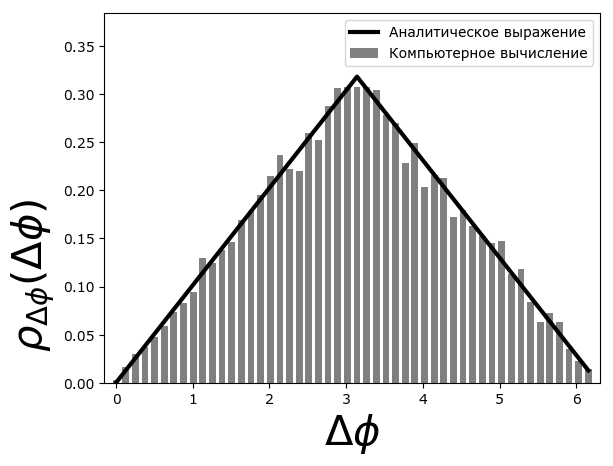
\includegraphics[width=1\linewidth]{const_alpha_10000}}
$N = 10^4$ \\
\end{minipage}
\hfill
\begin{minipage}[h]{0.47\linewidth}
\center{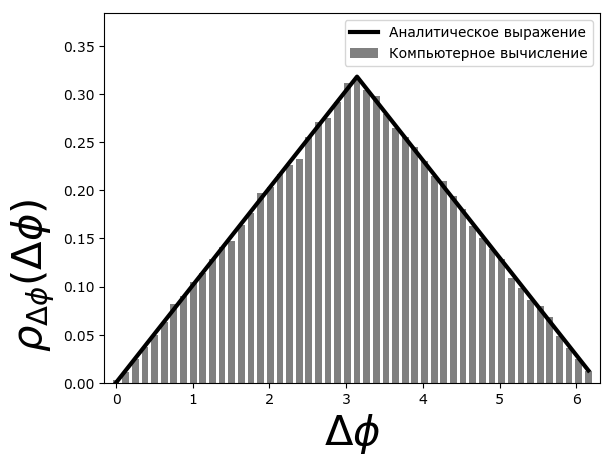
\includegraphics[width=1\linewidth]{const_alpha_100000}}
$N = 10^5$ \\
\end{minipage}
\vfill
\begin{minipage}[h]{0.47\linewidth}
\center{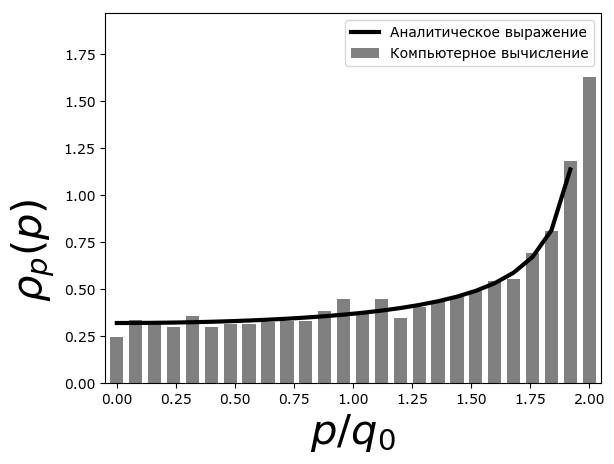
\includegraphics[width=1\linewidth]{const_momentum_10000}}
$N = 10^4$ \\
\end{minipage}
\hfill
\begin{minipage}[h]{0.47\linewidth}
\center{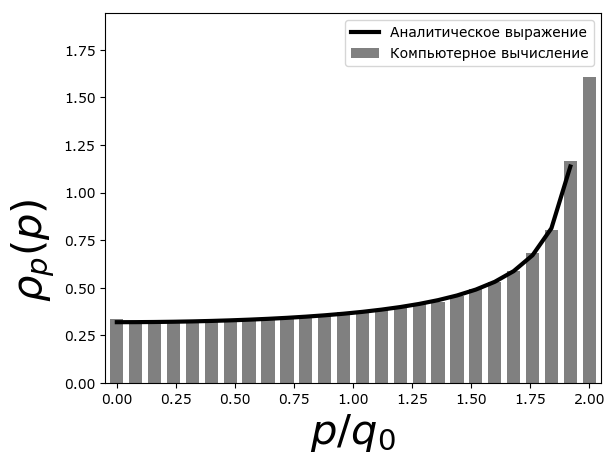
\includegraphics[width=1\linewidth]{const_momentum_100000}}
$N = 10^5$\\
\end{minipage}
\caption{Распределение по углу разлета и величине импульса в константном случае}
\label{const_fig}
\end{figure}

\subsection{Гауссов случай}
В случае нормального распределения импульса кварков импульс мезона и угол разлета определяются выражениями
\begin{eqnarray}
p = \sqrt{\br{q_2^x - q_1^x}^2 + \br{q_2^y - q_1^y}^2} \\
cos \Delta \phi = \frac{\vec{p_1} \cdot \vec{p_2}}{p_1 p_2}
\end{eqnarray}
Их распределения
\begin{gather}
\rho_p \br{p} = \frac{p \ e^{-\frac{p^2}{2q_0^2}}}{q_0^2} \\
\rho_{\Delta \phi} \br{\Delta \phi} = \frac{3}{8 \pi} \cdot \frac{\sqrt{1 - \br{\gamma / 2}^2} - \br{\gamma / 2} \ arccos \br{\gamma / 2}}{\br{1 - \br{\gamma/2}^2}^{3/2}}, \quad \text{где} \ \gamma = cos \Delta \phi
\end{gather}
Гистограммы распределений этих величин изображены на рисунке \ref{gauss_fig}.
\begin{figure}
\begin{minipage}[h]{0.47\linewidth}
\center{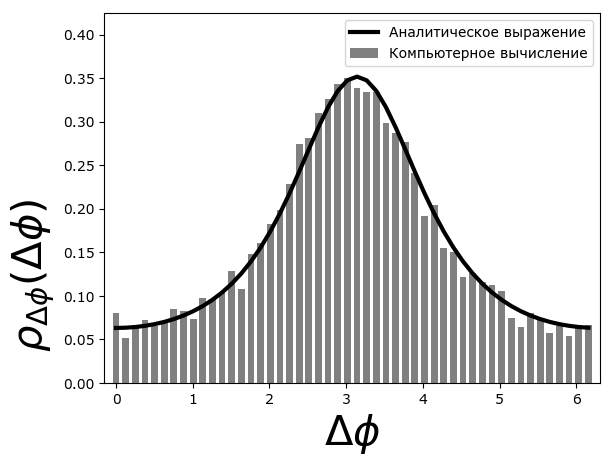
\includegraphics[width=1\linewidth]{gauss_alpha_10000}}
$N = 10^4$ \\
\end{minipage}
\hfill
\begin{minipage}[h]{0.47\linewidth}
\center{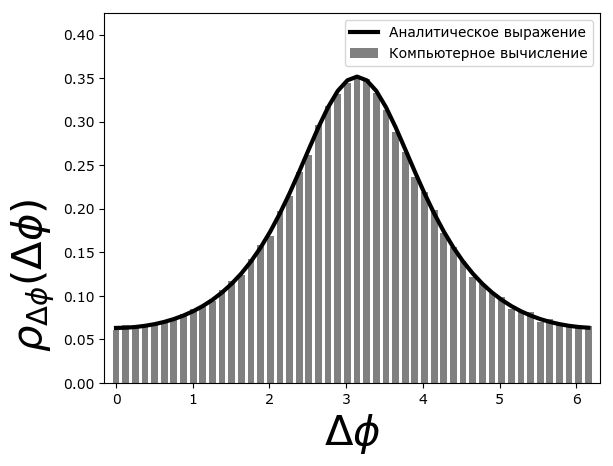
\includegraphics[width=1\linewidth]{gauss_alpha_100000}}
$N = 10^5$ \\
\end{minipage}
\vfill
\begin{minipage}[h]{0.47\linewidth}
\center{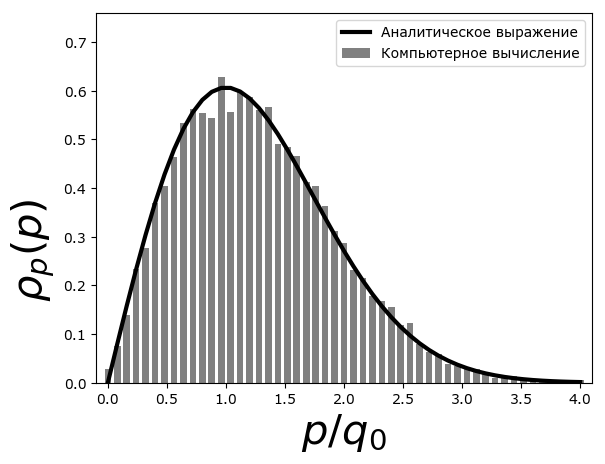
\includegraphics[width=1\linewidth]{gauss_momentum_10000}}
$N = 10^4$ \\
\end{minipage}
\hfill
\begin{minipage}[h]{0.47\linewidth}
\center{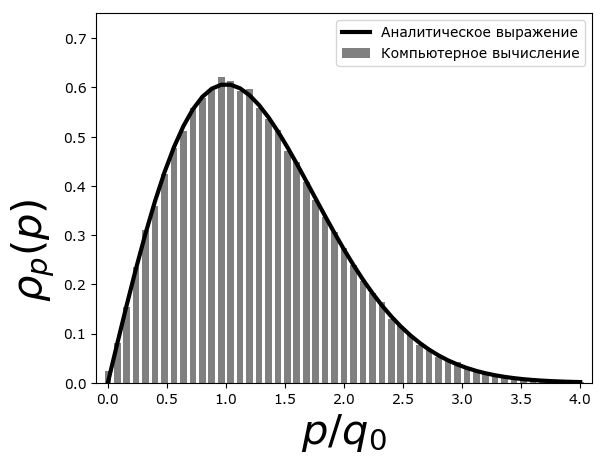
\includegraphics[width=1\linewidth]{gauss_momentum_100000}}
$N = 10^5$\\
\end{minipage}
\caption{Распределение по углу разлета и величине импульса в гауссовом случае}
\label{gauss_fig}
\end{figure}

\section{Заключение}
% \subsection{Импульсная корреляционная функция}
% В результате всех вычислений мы можем однозначно сказать, как выглядит импульсная часть двухчастичной корреляционной функции $G^2$. Как правило эту функцию определяют для наборов декартовых компонент импульса двух частиц $G^2 = G^2 \br{p_1^x, p_1^y, p_1^z, p_2^x, p_2^y, p_2^z}$. Вместо них мы воспользуемся величиной и направлением поперечных импульсов и быстротами:
% \begin{gather}
% G^2 = G^2 \br{p_1, p_2, \phi_1, \phi_2, \eta_1, \eta_2} = \rho_p \br{p_1} \cdot \rho_p \br{p_2} \cdot \rho_{\Delta \phi} \br{\phi_2 - \phi_1} \cdot \rho_\eta \br{\eta_1} \cdot \rho_\eta \br{\eta_2}.
% \end{gather}
% Функция $\rho_\eta$ для модели Артру-Меннессиера известна. Она равна константе для широкого интервала быстрот.

\subsection{Объяснение наличия заднего риджа}
В нашей модели появляется пик с центром $\Delta \phi = \pi$. Для полной функции распределения (на рис. \ref{main}), так как в среднем на одну частицу приходится одна единица быстроты и частицы от соседних струн в среднем разделены интервалом $\abs{\Delta \eta} = 1$, это означает появление двух холмов с центрами в точках $(\Delta \phi , \Delta \eta) = (\pi, -1)$ и $(\Delta \phi , \Delta \eta) = (\pi, 1)$. На рисунке мы видим их сильно "размазаными" по быстроте, то есть именно они и формируют задний ридж.
\appendix
\section{Код компьютерной программы для вычислений методом Монте-Карло}
Код исполняется интерпретатором языка Python 3.4+ и использует дополнительные модули: matplotlib и numpy.
\begin{verbatim}
import math
import numpy
import random
from numpy import pi
from functools import partial
import pylab
from matplotlib import mlab


def plot_theory_and_practice(x_list,
                             practice_list,
                             theory_list,
                             string_name,
                             picture_name):
    dx = x_list[1] - x_list[0]
    practice = pylab.bar(x_list, practice_list, width = 0.7 * dx,
                    align = "center", color="gray")
    theory = pylab.plot(x_list, theory_list, color="black", linewidth = 3)
    xlabel_ = pylab.xlabel("$" + string_name + "$")
    ylabel_ = pylab.ylabel(r"$\rho_{" + string_name + r"} \left( " + \
    string_name + r"\right)$")
    practice[0].set_label("Computer calculations")
    theory[0].set_label("Analitic calculations")
    xlabel_.set_size(20)
    ylabel_.set_rotation(1)
    ylabel_.set_size(20)
    ylabel_.set_horizontalalignment("right")
    pylab.legend()
    #pylab.show()
    pylab.savefig(picture_name + ".png", bbox_inches='tight')
    pylab.close()


def plot_distribution(*,
                      string_name,
                      calculate_function,
                      theory_function,
                      left_bound,
                      right_bound,
                      da,
                      N,
                      picture_name):
    a_list = numpy.array([left_bound + i * da
                          for i in range(int((right_bound - left_bound) / da) + 1)])
    dN_list = numpy.zeros(a_list.shape)
    for i in range(N):
        a = calculate_function()
        n = round((a - left_bound) / da)
        if 0 <= n < len(dN_list):
            dN_list[n] += 1
    dN_list[0] *= 2
   
    rho_a_practice = dN_list / (da * N)
    rho_a_theory = numpy.array([theory_function(a) for a in a_list])
    plot_theory_and_practice(a_list, rho_a_practice, rho_a_theory, string_name, \
    picture_name + "_" + str(N))


def rand_angle():
    return (2 *random.random() - 1) * pi


def gauss_momentum_component(q0):
    return random.normalvariate(0.0, q0 / math.sqrt(2))

    
def gauss_momentum(q0):
    qx = gauss_momentum_component(q0)
    qy = gauss_momentum_component(q0)
    return math.sqrt(qx * qx + qy * qy)


def const_theory_alpha_distribution(a):
    if a <= pi:
        return a / (pi * pi)
    elif pi < a <= 2 * pi:
        return (2 * pi - a) / (pi * pi)
    return 0.0

    
def const_theory_momentum_distribution(p):
    rho = p / (2 * q0)
    if rho >= 1.0:
        return numpy.nan
    return (2 / pi) * (1 / (2 * q0)) * (1 / math.sqrt(1.0 -  rho * rho))


def gauss_theory_alpha_distribution(a):
    y = math.cos(a)
    c = math.sqrt(1 - y * y / 4)
    return (3 / (8 * pi)) * (c - (y / 2) * math.acos(y / 2)) / (c ** 3)


def get_alpha_const():
    f1 = rand_angle()
    f2 = rand_angle()
    f3 = rand_angle()
    f = 1 if (f3 - f2) * (f2 - f1) >= 0 else 0  
    alpha = (2 * f - 1) * abs(f3 - f1) / 2 + (1 - f) * pi
    alpha = pi + random.choice((-1, 1)) * (pi -alpha)
    return alpha


def get_momentum_const(q0):
    f1 = rand_angle()
    f2 = rand_angle()
    return 2 * q0 * abs(math.cos((f2 - f1) / 2.0))


def get_momentum_gauss(q0):
    q1 = gauss_momentum(q0)
    q2 = gauss_momentum(q0)
    f1 = rand_angle()
    f2 = rand_angle()
    return math.sqrt(q1 * q1 + q2 * q2 - 2 * q1 * q2 * math.cos(f2 - f1))


def get_alpha_gauss(q0):
    q1x = gauss_momentum_component(q0)
    q2x = gauss_momentum_component(q0)
    q3x = gauss_momentum_component(q0)
    q1y = gauss_momentum_component(q0)
    q2y = gauss_momentum_component(q0)
    q3y = gauss_momentum_component(q0)
    p1x = q2x - q1x
    p2x = q3x - q2x
    p1y = q2y - q1y
    p2y = q3y - q2y
    p1 = math.sqrt(p1x * p1x + p1y * p1y)
    p2 = math.sqrt(p2x * p2x + p2y * p2y)
    alpha = math.acos((p1x * p2x + p1y  * p2y) / (p1 * p2))
    alpha = pi + random.choice((-1, 1)) * (pi -alpha)
    return alpha


q0 = 1.0
plot_distribution = partial(plot_distribution, N=100000,
                            calculate_function=lambda: 0,
                            theory_function=lambda x: numpy.nan)
plot_alpha_distribution = partial(plot_distribution, string_name=r"\Delta \phi",
                                  left_bound=0, right_bound=2 * pi, da=2*pi/50)
plot_momentum_distribution = partial(plot_distribution, string_name=r"p",
                                     left_bound=0.0, right_bound=2*q0, da=2*q0/25)

## CONST
plot_alpha_distribution(calculate_function=get_alpha_const,
                        theory_function=const_theory_alpha_distribution,
                        picture_name="const_alpha")         

plot_momentum_distribution(calculate_function=partial(get_momentum_const, q0),
                           theory_function=const_theory_momentum_distribution,
                           picture_name="const_momentum")


## GAUSS
plot_momentum_distribution(calculate_function=partial(get_momentum_gauss, q0),
                           theory_function= \
                           lambda p: p * math.exp(-(p * p) / (2 * q0 * q0)) / q0 /q0,
                           right_bound=4*q0,
                           picture_name="gauss_momentum")

plot_alpha_distribution(calculate_function=partial(get_alpha_gauss, q0),
                        theory_function=gauss_theory_alpha_distribution,
                        picture_name="gauss_alpha")
\end{verbatim}



\newpage
\section*{}
\addcontentsline{toc}{section}{Список литературы}
\begin{thebibliography}{00}
\bibitem{model1}
A. B. Kaidalov, Phys. Lett. B 116, p.459 (1982).
\bibitem{model2}
A. B. Kaidalov, K. A. Ter-Martirosyan, Phys. Lett. B 117 p.247 (1982).
\bibitem{model3}
A. Cappela, U. Sukhatme, Chung-I Tan, J. Tran Thanh Van, Phys. Lett. B 81, 68 (1979).
\bibitem{model4}
A. Cappela, U. Sukhatme, Chung-I Tan, J. Tran Thanh Van, Phys. Rep. 236 p.225 (1994).
\bibitem{nesterenko}
Барбашов Б. М., Нестеренко В. В. Модель релятивистской струны в физике адронов, М.: Энергоиздат, 1987.
\bibitem{schwinger}
J. Schwinger, Phys. Rev. 82, p.664 (1951).
\bibitem{artru}
X. Artru, Phys. Rep. 97, p.147 (1983).
\bibitem{fragmentation_lit}
V. V. Vechernin, arXiv: 0812.0604 [hep-ph].
\bibitem{cappela}
A. Capella, A. Krzywicki, Phys. Rev. D 18 p.4120 (1978).
\bibitem{exp_data}
{\bf ALICE} Collaboration, B. Abelev \textit{et al.}, arxiv:1307.3237 [nucl-ex].
\bibitem{fusion1}
M. A. Braun, C. Pajares, Phys. Lett. B 287, p.154 (1992).
\bibitem{fusion2}
M. A. Braun, C. Pajares, Nucl. Phys. B 390, p.542 (1993).
\bibitem{fusion_corr1}
N. S. Amelin, N. Armesto, M. A. Brown, E. G. Ferreiro, C. Pajares, Phys. Rev. Lett. 73, p.2813 (1994).
\bibitem{fusion_corr2}
M. A. Braun, R. S. Kolevatov, C. Pajares, V. V. Vechernin, Eur.Phys. J. C 32, p.535 (2004); arXiv:hep-ph/0307056.
\bibitem{fusion_corr3}
V. V. Vechernin, R. S. Kolevatov, Phys. Atom. Nucl. 70 p.1797 (2007).
\bibitem{fusion_corr4}
V. V. Vechernin, R. S. Kolevatov, Phys. Atom. Nucl. 70 p.1809 (2007).
\bibitem{venus}
K. Werner, Phys. Rep. 232, p.87 (1993).
\end{thebibliography}


\end{document}